\documentclass[reqno]{amsart}
\usepackage[utf8]{inputenc}
\usepackage[top=1.4in, bottom=1.2in, left=1.2in, right=1.2in]{geometry}

\usepackage{amssymb,amsfonts,amsmath,amsthm,tikz,tikz-cd,graphicx,url,mathtools}
\usetikzlibrary{arrows.meta}
\usepackage[mode=buildnew]{standalone}
\usepackage{xcolor}
\usepackage[all,arc]{xy}
\usepackage{enumerate}
\usepackage[colorlinks=true]{hyperref}
\usepackage[alphabetic]{amsrefs}
\usepackage{comment}
\usepackage{subfigure}
\usetikzlibrary{matrix}
\usepackage{cmap}
\usepackage{xparse}
\usepackage{stmaryrd}

\usepackage[sc,osf]{mathpazo}
\usepackage{upgreek}
\usepackage{optparams,eurosym}

\newtheorem{thm}{Theorem}[section]
\newtheorem{cor}[thm]{Corollary}
\newtheorem{prop}[thm]{Proposition}
\newtheorem{lem}[thm]{Lemma}
\newtheorem{conj}[thm]{Conjecture}
\newtheorem{quest}[thm]{Question}

\theoremstyle{definition}
\newtheorem{defn}[thm]{Definition}
\newtheorem{defns}[thm]{Definitions}
\newtheorem{con}[thm]{Construction}
\newtheorem{exmp}[thm]{Example}
\newtheorem{exmps}[thm]{Examples}
\newtheorem{notn}[thm]{Notation}
\newtheorem{notns}[thm]{Notations}
\newtheorem{addm}[thm]{Addendum}
\newtheorem{exer}[thm]{Exercise}
\newtheorem{fact}[thm]{Fact}
\newtheorem*{claim}{Claim}

\theoremstyle{remark}
\newtheorem{rem}[thm]{Remark}
\newtheorem{rems}[thm]{Remarks}
\newtheorem{warn}[thm]{Warning}
\newtheorem{sch}[thm]{Scholium}

\newcommand{\tinypar}[1]{\marginpar{\parbox[b]{\marginparwidth}{\tiny#1}}}

\newcommand{\Z}{\mathbb Z}
\newcommand{\RP}{\mathbb{RP}}
\newcommand{\ZZ}{\mathbb{Z}/2}
\newcommand{\QQ}{\mathbb{Q}}
\newcommand{\RR}{\mathbb{R}}
\newcommand{\FF}{\mathbb{F}}
\newcommand{\gl}{\mathfrak{gl}}
\newcommand{\CP}{\mathbb{CP}}
\newcommand{\nm}[1]{\left\|#1\right\|}
\newcommand{\innp}[2]{\langle #1,#2\rangle}

\newcommand{\cat}{\mathcal{T}}
\newcommand{\cak}{\mathcal{K}}
\newcommand{\whc}{\widehat{\chi}}

\DeclareMathOperator{\dimm}{dim}
\DeclareMathOperator{\degg}{deg}
\DeclareMathOperator{\pt}{pt}
\DeclareMathOperator{\idd}{id}
\DeclareMathOperator{\Cone}{Cone}
\DeclareMathOperator{\CKhI}{CKhI}
\DeclareMathOperator{\KR}{KR}
\DeclareMathOperator{\Kh}{Kh}
\DeclareMathOperator{\KhIr}{\widetilde{KhI}}
\DeclareMathOperator{\CKh}{CKh}
\newcommand{\Khr}{\widetilde{\Kh}}
\newcommand{\lra}[1]{\langle #1 \rangle}
\newcommand{\lrb}[1]{\llbracket #1 \rrbracket}

\title{The Gorsky--Oblomkov--Rasmussen conjecture over $\mathbb{Q}$}


\author{Qiuyu Ren}
\email{qren18@stanford.edu}
\address{Department of Mathematics, Stanford University, Stanford, CA 94305}


\author{Hongjian Yang}
\email{yhj@stanford.edu}
\address{Department of Mathematics, Stanford University, Stanford, CA 94305}


\subjclass[2020]{57K18, 13D02, 13D40}
\keywords{Gorsky--Oblomkov--Rasmussen conjecture, $\mathfrak{gl}_N$ homology, Koszul algebra, torus link}
\date{\today}



\begin{document}

\begin{abstract}
  We prove a generation theorem for the homology of certain Koszul complexes which naturally arise as the $E^1$ pages of the stable Rasmussen spectral sequence of torus links. Combining this theorem with recent work of Ballinger, Gorsky, Hogancamp, and Wang, we compute the stable Khovanov--Rozansky $\mathfrak{gl}_N$ homology of torus links and determine its Poincar\'e series, resolving conjectures of Gorsky, Oblomkov, and Rasmussen and their $\mathfrak{gl}_N$ analogs, over $\mathbb{Q}$. Using these results, we determine the Khovanov homology of $T(n,n-1)$ and $T(n,n)$ over $\mathbb{Q}$, confirming conjectures of Shumakovitch and Turner and of the first author, which in turn allows us to compute the Khovanov skein lasagna module of $\overline{\mathbb{CP}^2}$ over $\mathbb{Q}$.
\end{abstract}

\maketitle


\section{Introduction}
Jones polynomials of torus links $T(n,m)$ have well-known closed formulas. In contrast, the Khovanov homology of torus links is notoriously hard to compute. Complete calculations for torus links on at most three strands are given in \cite{khovanov2000categorification,turner2008spectral,stosic2009khovanov,gillam2012knot}, but no computations for an infinite family are known beyond these cases.

By the work of Sto\v{s}i\'{c} \cite{stosic2007homological,stosic2009khovanov}, after suitable grading shifts, the Khovanov homology, or more generally, the Khovanov--Rozansky $\mathfrak{gl}_N$ homology, of $T(n,m)$ has a stable limit as $m\to\infty$, which we call the homology of $T(n,\infty)$. A conjectural formula for the Khovanov--Rozansky $\mathfrak{gl}_N$ homology of $T(n,\infty)$ was proposed in Gorsky--Oblomkov--Rasmussen \cite{gorsky2013stable} and some subsequent papers \cite{gorsky2014torus,gorsky2015stable}.
\begin{conj}\label{conj:GOR}
The Khovanov--Rozansky $\mathfrak{gl}_N$ homology of $T(n,\infty)$ is isomorphic to the homology of the DGA $K_{n,\Z}:=(\Z[u_0,\cdots,u_{n-1}]\otimes\wedge(\xi_0,\cdots,\xi_{n-1}),d_N)$, where $$d_Nu_k=0,\ d_N\xi_k=\sum_{\substack{0\le i_1,\cdots,i_N<n\\i_1+\cdots+i_N=k}}u_{i_1}\cdots u_{i_N}.$$ Here, $u_k$, $\xi_k$ have (cohomological, quantum) degrees $(-2k,2k+2)$, $(-2k-1,2k+2N)$, respectively.
\end{conj}

Recently, over rational coefficients, Ballinger, Gorsky, Hogancamp, and Wang \cite[Theorem~1.1 and Remark~1.4]{ballinger2025stable} reduced this conjecture to a purely algebraic generation question, which we answer affirmatively below.

Let $K_n:=K_{n,\Z}\otimes\QQ$ denote the rationalization of the DGA $K_{n,\Z}$. For $1\le k\le n-1$, define \[\mu_k=\sum_{i+j=k}(Ni-j)u_i\xi_j\in K_n.\] One can check that they are cycles in $K_n$.

Our first main result is the following generation theorem for the homology of $K_n$, which proves \cite[Conjecture~1.1]{gorsky2013stable} and \cite[Conjecture~1]{gorsky2015stable} over $\QQ$.

\begin{thm}\label{thm:Koszul generation}
For every $n\ge1$ and $N\ge1$, the homology $H_*(K_n)$ is generated by $[\mu_1],\cdots,[\mu_{n-1}]$ as an algebra over $\QQ[u_0,\cdots,u_{n-1}]$. Consequently, by \cite[Theorem~1.1 and Section~7.1]{ballinger2025stable}, the Khovanov--Rozansky homology of $T(n,\infty)$ over $\QQ$ is isomorphic to $H_*(K_n)$ as a bigraded vector space.
\end{thm}

Bai, Gorsky, and Kivinen \cite{bai2020quadratic} proved Theorem~\ref{thm:Koszul generation} for $N=2$ and in Koszul degree 1. However, induction on $n$ alone does not seem to suffice to prove Theorem~\ref{thm:Koszul generation} for all Koszul degrees since proceeding from $n$ to $n+1$ requires more knowledge of the structure of the Koszul complex than the induction hypothesis provides. For a fixed $N\ge1$, our proof of Theorem~\ref{thm:Koszul generation} instead introduces an auxiliary two-parameter family of DGAs $\mathcal K_{r,l}$ with $\cak_{n,(N-1)n}\cong K_n$, and inducts on a generalized finite generation statement. In appropriate ranges, there is an exact sequence
\begin{equation}\label{eq:exact_sequence}
0\to H_*(\mathcal K_{r-1,l})\to H_*(\mathcal K_{r,l})\to H_*(\mathcal K_{r,l-1})\to0
\end{equation}
in which the second map is an algebra map. This enables us to perform the induction step by reducing the generation statement for $\mathcal K_{r,l}$ to a finite check. In addition, the exact sequence \eqref{eq:exact_sequence} enables us to compute the Poincar\'e series of the homology of $T(n,\infty)$ inductively.

Variants of Theorem~\ref{thm:Koszul generation} for deformed potentials and reduced homology are given in Corollaries~\ref{cor:deformed} and~\ref{cor:reduced}.

The homology of $T(n,\infty)$ is a direct limit of the homology of $T(n,m)$ along maps induced by cobordisms $T(n,m)\to T(n,m+1)$ that each create $n-1$ saddles. By symmetry of $n,m$, there are also maps from $T(n,m)$ to $T(n+1,m)$. All squares formed by these cobordism maps commute up to isotopy. We define the $\mathfrak{gl}_N$ homology of $T(\infty,\infty)$ as the colimit of that of $T(n,m)$ as $n,m\to\infty$. In Section~\ref{sec:stable torus homology}, we prove stabilization of this colimit, and in Appendix~\ref{app:Hilbert series}, we give a formula for its Poincar\'e series. The following theorem summarizes the main results in Appendix~\ref{app:Hilbert series}, which confirms and generalizes \cite[Conjectures~1.7 and 4.9]{gorsky2013stable}.

\begin{thm}\label{thm:stable Hilbert series}
For every $n\ge1$ and $N\ge1$, Theorem~\ref{thm:finite Hilbert series} gives a closed formula for the complete bigraded Poincar\'e series of the Khovanov--Rozansky $\gl_N$ homology of $T(n,\infty)$. Theorem~\ref{thm:fermionic formula} gives a closed formula for $T(\infty,\infty)$.
\end{thm}


In the case $N=2$, Shumakovitch and Turner (see \cite[Conjecture~1.8]{gorsky2013stable}) conjectured a formula for the Khovanov homology of torus knots $T(n,n-1)$ over the rationals, and the first author \cite[Conjectures~6.1 and~6.1\(^{\prime}\)]{ren2024lee} proposed one for torus links $T(n,n)$. As noted in \cite{ren2024khovanov}, the formula for $T(n,n)$ implies a complete determination of the Khovanov skein lasagna modules \cite{morrison2022invariants} of the manifold $\overline{\CP^2}$ over the rationals, which appears in terms of closed form Poincar\'e series in Ritter von Merkl \cite[Section~4.1]{ritter2025computing}.

Combining Theorem~\ref{thm:stable Hilbert series} and the idea in \cite[Section~1.6.2]{ren2026khovanov}, we prove these conjectures. We state the resulting formulas in the conventions of \cite{ren2024lee,ren2024khovanov}.

\begin{thm}\label{thm:finite torus links and lasagna}
\begin{enumerate}
\item Let $A_n(t,q)$ denote the Poincar\'e polynomial of $\Kh(T(n,n-1);\QQ)$ for $n\ge1$. Then,
\[
A_1=A_2=q^{-1}+q,\ A_3=q+q^3+t^2q^5+t^3q^9,
\]
and, for $n\ge4$,
\[
A_n=q^{2n-4}A_{n-1}+t^{2n-4}q^{6n-12}A_{n-2}
+t^{2n-3}q^{8n-16}A_{n-3}.
\]
\item Let $I_n(t,q)$ denote the Poincar\'e polynomial of $\Kh(T(n,n);\QQ)^{S_n}$ for the $S_n$-action induced by braiding the cable strands (see \cite{grigsby2018annular}), for $n\ge0$. Then,
\[
I_n=\sum_{i=0}^{\lfloor(n-1)/2\rfloor}
 t^{2i(n-i)}q^{6i(n-i)+n-4i-1}A_{n-2i}+\begin{cases}
 t^{n^2/2}q^{3n^2/2-n},&n\text{ even},\\
 0,&n\text{ odd}.
\end{cases}
\]
\item Let $B_n(t,q)$ denote the Poincar\'e polynomial of $\Kh(T(n,n);\QQ)$ for $n\ge0$. Then,
\[
B_n=\sum_{i=0}^{\lfloor n/2\rfloor}
\left(\binom{n}{i}-\binom{n}{i-1}\right)
 t^{2i(n-i)}q^{6i(n-i)}I_{n-2i},
\]
where $\binom{n}{-1}=0$.
\item Let $\mathcal L_\alpha(t,q)$ denote the Poincar\'e series of the $\mathfrak{gl}_2$ skein lasagna module $\mathcal S_0^2(\overline{\CP^2};\alpha;\QQ)$, using the grading conventions of \cite{ren2024khovanov}, and identify $H_2(\overline{\CP^2};\Z)$ with $\mathbb Z$ by sending $[\overline{\CP^1}]$ to $1$. Then,
\begin{align}
\mathcal L_0(t,q)
&=1+\sum_{r=1}^{\infty}t^{-2r^2}q^{6r^2-4r+1}A_{2r}(t,q^{-1}),
\label{eqn:intro lasagna zero}\\
\mathcal L_1(t,q)
&=\sum_{r=1}^{\infty}t^{-2r^2+2r}q^{6r^2-10r+4}A_{2r-1}(t,q^{-1}).
\label{eqn:intro lasagna one}
\end{align}
More generally, for any $\alpha\in\Z$, let $\epsilon\in\{0,1\}$ be its residue modulo $2$. Then we have
\[
\mathcal L_\alpha(t,q)
=t^{(\alpha^2-\epsilon)/2}q^{-(\alpha^2-\epsilon)/2}\mathcal L_\epsilon(t,q).
\]
\end{enumerate}
\end{thm}


Items (1), (2)+(3), and (4) of Theorem~\ref{thm:finite torus links and lasagna} confirm \cite[Conjecture 1.8]{gorsky2013stable}, \cite[Conjecture 6.1]{ren2024lee}, and \cite[Conjecture 6.15]{ren2024khovanov} respectively. The series \eqref{eqn:intro lasagna zero} agrees with the even closed formula in \cite[Conjecture~4.3]{ritter2025computing}. To obtain \eqref{eqn:intro lasagna one} in the grading convention of \cite{ren2024khovanov}, the odd closed formula there must be multiplied by $q$.

\subsection*{Organization of the paper}We prove Theorem~\ref{thm:Koszul generation} in Section~\ref{sec:Koszul generation} and put it into link homology context in Section~\ref{sec:stable torus homology}. In Section~\ref{sec:unstable}, we prove Theorem~\ref{thm:finite torus links and lasagna}. In Appendix~\ref{app:Hilbert series}, we give a closed formula for the Poincar\'e series of the stable homology of torus links, proving Theorem~\ref{thm:stable Hilbert series}.

\subsection*{AI disclosure}The idea of introducing an auxiliary family in Section~\ref{sec:Koszul generation} was initially proposed by the authors and largely developed by AI. In particular, AI found and proved the identity \eqref{eqn:identity for Omega_T}, crucial to complete the induction. AI also carried out the computations in Section~\ref{sec:variants} and Appendix~\ref{app:Hilbert series}, and assisted with the write-up. The authors then checked and substantially simplified the proof. AI also helped with minor editorial tasks.

\subsection*{Lean formalization}AI-generated Lean~4 formalizations of Theorems~\ref{thm:Koszul generation},~\ref{thm:finite Hilbert series}, and~\ref{thm:fermionic formula} are available at \cite{stable_torus_link_homology}.

\subsection*{Acknowledgements}We thank Eugene Gorsky and Ciprian Manolescu for helpful discussions and comments on an earlier version of this draft. We also thank the organizers of the long program Quantum Topology, Character Varieties and Low-Dimensional Geometry and IPAM for hosting us. This work was conducted during the period when QR served as a Clay Research Fellow. HY was partially supported by the Simons Collaboration grant on New Structures in Low-Dimensional Topology and a Simons Dissertation Fellowship. 

\section{Proof of Theorem~\ref{thm:Koszul generation}}\label{sec:Koszul generation}

\subsection{A two-parameter family of Koszul complexes}

We first fix some conventions. All tensor products are over $\QQ$ unless otherwise specified. For a commutative $\QQ$-algebra $R$ and $r_1,\dots,r_m\in R$, we define a supercommutative differential graded algebra (DGA) $K_R(r_1,\dots,r_m)$ as the Koszul complex \[K_R(r_1,\dots,r_m)\coloneqq R\otimes\wedge(\xi_1,\dots,\xi_m),\ du=0\ (u\in R),\ d\xi_i=r_i.\]
The Koszul degree is defined by declaring that $\xi_i$ has degree $1$ and elements in $R$ have degree $0$. The differential extends by the graded Leibniz rule.

For a formal Laurent series $f(z)$ with coefficients in a DGA, we write $[z^k]f$ for its coefficient of $z^k$ and set $D=z\,d/dz$, so $[z^k]Df=k[z^k]f$. We take $z$ to be even with $dz=0$. The differential acts coefficientwise and commutes with $D$. The parity of an element is its Koszul degree modulo $2$; a series is odd (resp. even) if all its coefficients are odd (resp. even).

For nonnegative integers $r,l$, we define $S_r=\QQ[e_1,\dots,e_r]$, and
\[e(z)=1+\sum_{i=1}^r e_i z^i,\ G_j=[z^j]e(z)^N\in S_r.\]
We set $e_0=1$, $e_i=0$ for $i<0$ or $i>r$, and $G_j=0$ for $j<0$. Taking the coefficient of $z^j$ in $eD(e^N)=N(De)e^N$ gives
\begin{equation}\label{eqn:recurrence for G_j}G_j=\frac{1}{j}\sum_{i=1}^r\bigl((N+1)i-j\bigr)e_iG_{j-i}\ (j\ge1).
\end{equation}

We define $\cak_{r,l}$ to be the supercommutative DGA over $S_r$ generated by elements $\whc_j^{r,l}$ of Koszul degree $1$ for $j>l$, subject to the relations \begin{equation}\label{eqn:defn of whc_j}
\whc_j^{r,l}=\frac{1}{j}\sum_{i=1}^r\bigl((N+1)i-j\bigr)e_i\whc_{j-i}^{r,l}\ (j>l+r),
\end{equation}with differential $de_i=0$ and $d\whc_j^{r,l}=G_j$. Here $\whc_j^{r,l}=0$ for $j\le l$. The recurrence \eqref{eqn:recurrence for G_j} shows that the differential respects these relations. We omit the superscripts $r,l$ from the notation when they are clear from the context.

The relations express each $\whc_j$ with $j>l+r$ uniquely as a linear combination of $\whc_{l+1},\dots,\whc_{l+r}$ over $S_r$. Writing $\chi_j=\whc_j$ for $l<j\le l+r$, we therefore have
\[\cak_{r,l}=K_{S_r}(G_{l+1},\dots,G_{l+r}).\]


For $j>\max\{l,Nr\}$, the generator $\whc_j$ is closed since $G_j=0$, and we call it a \emph{tail cycle}. Let $\cat_{r,l}\subset H_*(\cak_{r,l})$ be the subalgebra generated by the tail cycles $[\whc_j]$ ($j>\max\{l,Nr\}$) over $S_r$. The main theorem of this section is the following.

\begin{thm}\label{thm:2 parameter Koszul generation}
  $\cat_{r,l}=H_*(\cak_{r,l})$ for all $r,l\ge 0$.
\end{thm}


\begin{rem}When $l<Nr$, the assertion is equivalent to saying that $H_*(\cak_{r,l})$ is generated over $S_r$ by the tail cycles $\whc_{Nr+1},\dots,\whc_{Nr+r-1}$. In fact, $\whc_{Nr+r}$ is a linear combination of $\whc_{Nr+1},\dots,\whc_{Nr+r-1}$ since the $i=r$ term in the recurrence relation \eqref{eqn:defn of whc_j} vanishes. The recurrence then expresses all higher tail cycles as linear combinations of these.
\end{rem}

\begin{exmp}
Take $N=2$ and $r=l=2$. Then $\cak_{2,2}$ is defined by the relations
\[d\chi_3=2e_1e_2,\ d\chi_4=e_2^2,\ \whc_5=(e_2\chi_3-2e_1\chi_4)/5.\]
We check directly that
\[d\whc_5=(2e_1e_2^2-2e_1e_2^2)/5=0.\]
For $f,g\in S_2$, we have
\[d(f\chi_3+g\chi_4)=e_2(2e_1f+e_2g),\]
which vanishes exactly when $f=e_2h$ and $g=-2e_1h$ for some $h\in S_2$. Thus the $1$-cycles are given by $S_2\whc_5$. Moreover, we have $d(\chi_3\chi_4)=-5e_2\whc_5$, so the $1$-boundaries are given by $e_2S_2\whc_5$. Together with $H_0=S_2/(e_1e_2,e_2^2)$ and $H_2=0$, we obtain
\[H_*(\cak_{2,2})\cong(S_2\otimes\wedge([\whc_5]))/(e_1e_2,e_2^2,e_2[\whc_5]).\]
Thus the homology can be generated by the tail class $[\whc_5]$.
\end{exmp}




We first explain how Theorem~\ref{thm:2 parameter Koszul generation} implies Theorem~\ref{thm:Koszul generation}. We use the convention $K_0=\QQ$.

\begin{prop}\label{prop:Krl in terms of Km}
For $r\ge1$ and $0\le m\le r$, there is a DGA isomorphism
\[
\cak_{r,Nr-m}\cong K_m\otimes\QQ[e_1,\dots,e_{r-m}]\otimes\wedge(\chi_{Nr+1},\dots,\chi_{(N+1)r-m}),
\]
where the last two factors have zero differential. This isomorphism identifies
$u_i$ with $e_{r-i}$ and $\xi_i$ with $\chi_{Nr-i}$ for $0\le i<m$.
In particular, $K_n\cong\cak_{n,(N-1)n}$.
\end{prop}

\begin{proof}
Using the Koszul description, we have
\[\cak_{r,Nr-m}=K_{S_r}(G_{Nr-m+1},\dots,G_{Nr})\otimes\wedge(\chi_{Nr+1},\dots,\chi_{Nr+r-m}),\]
where the second factor has zero differential. Since
\[[z^i](z^re(z^{-1}))^N=G_{Nr-i},\]
for $0\le i<m\le r$, only the first $m$ coefficients $e_r,\dots,e_{r-m+1}$ of $z^re(z^{-1})$ contribute to $G_{Nr-i}$. Thus the first factor is $K_m\otimes\QQ[e_1,\dots,e_{r-m}]$ under the stated identification of generators.
\end{proof}

Theorem~\ref{thm:2 parameter Koszul generation} implies Theorem~\ref{thm:Koszul generation}, as the following lemma explains.

\begin{lem}\label{lem:mu_k closed and tail generators}
For every $n\ge1$, the elements $\mu_1,\dots,\mu_{n-1}$ are closed in $K_n$. Under the isomorphism $K_n\cong\cak_{n,(N-1)n}$ of Proposition~\ref{prop:Krl in terms of Km}, they generate the same subalgebra of homology over $S_n$ as the tail classes $[\whc_{Nn+1}],\dots,[\whc_{Nn+n-1}]$.
\end{lem}

\begin{proof}
Set $r=m=n$ in Proposition~\ref{prop:Krl in terms of Km}. For $1\le k<n$, put $k'=Nn+n-k$. Under this isomorphism, we have
\[\mu_k=\sum_{n-k\le i\le n}(k'-(N+1)i)e_i\chi_{k'-i} =-k'\whc_{k'}-\sum_{1\le i<n-k}(k'-(N+1)i)e_i\whc_{k'-i}.\]
The second equality follows from \eqref{eqn:defn of whc_j}. Every $\whc_j$ on the right has $j>Nn$ and is closed, so $d\mu_k=0$. The transition matrix between $\mu_{n-1},\dots,\mu_1$ and $\whc_{Nn+1},\dots,\whc_{Nn+n-1}$ is upper triangular with invertible diagonal entries $-k'$, so their classes generate the same subalgebra of homology over $S_n$.
\end{proof}

\subsection{The induction step}

We prove Theorem~\ref{thm:2 parameter Koszul generation} by induction on $r+l$. Denote its assertion for $r,l\ge0$ by $P(r,l)$. We first check the following base cases.

\begin{lem}\label{lem:base cases of induction}
$P(r,l)$ holds when $l\ge Nr$ or $l=0$.
\end{lem}

\begin{proof}
When $l\ge Nr$, the differential is zero and the free generators $\chi_{l+1},\dots,\chi_{l+r}$ are tail cycles, so the assertion follows.
When $l=0$, the complex is the Koszul complex of the sequence $G_1,\dots,G_r$. Note that
\[G_j-Ne_j\in\QQ[e_1,\dots,e_{j-1}]\]
for $1\le j\le r$. We can solve successively for $e_1,\dots,e_r$ in terms of $G_1,\dots,G_r$, so $S_r=\QQ[G_1,\dots,G_r]$. Therefore, $\cak_{r,0}$ is a tensor product of complexes
\[\bigl(\QQ[G_j]\otimes\wedge(\chi_j),\ d\chi_j=G_j\bigr),\]
and hence its homology is concentrated in degree zero.
\end{proof}

Now assume that $0<l<Nr$. The defining relations of $\cak_{r,l}$ give two natural DGA maps
\[J\colon\cak_{r,l}\to\cak_{r,l-1},\ \rho\colon\cak_{r,l}\to\cak_{r-1,l}.\]
The map $J$ is the identity on $S_r$ and sends each generator to the generator with the same index:
\begin{equation}\label{eqn:J preserves tail classes}
J(\whc_j^{r,l})=\whc_j^{r,l-1}\ (j>l).
\end{equation}
The map $\rho$ sets $e_r=0$, fixes $e_1,\dots,e_{r-1}$, and satisfies
\begin{equation}\label{eqn:rho preserves tail classes}
\rho(\whc_j^{r,l})=\whc_j^{r-1,l}\ (j>l).
\end{equation}
Both maps respect the recurrence relations and commute with $d$. The following exact sequence relates $\cak_{r,l}$ with $\cak_{r,l-1}$ and $\cak_{r-1,l}$. Recall that $(C[1])_h=C_{h-1}$ and $d_{C[1]}=-d_C$.

\begin{prop}\label{prop:exact sequence for Krl}
There is a short exact sequence of chain complexes
\[0\to\cak_{r,l}\xrightarrow{J}\cak_{r,l-1}\xrightarrow{\pi}\cak_{r-1,l}[1]\to0.\]
It induces a long exact sequence in homology:
\begin{equation}\label{eqn:long exact sequence in homology}
\cdots\to H_*(\cak_{r-1,l})\xrightarrow{\delta}H_*(\cak_{r,l})\xrightarrow{J_*}H_*(\cak_{r,l-1})\to\cdots.
\end{equation}
Moreover, we have $\pi(cJ(b))=\pi(c)\rho(b)$ for $c\in\cak_{r,l-1}$ and $b\in\cak_{r,l}$.
\end{prop}

\begin{proof}
Let $C_0=K_{S_r}(G_{l+1},\dots,G_{l+r-1})$, regarded as a common sub-DGA of $\cak_{r,l}$ and $\cak_{r,l-1}$. As graded $S_r$-modules, we have decompositions \[\cak_{r,l}=C_0\oplus\chi_{l+r}C_0,\qquad \cak_{r,l-1}=C_0\oplus\chi_lC_0.\] The map $J$ is the identity on $C_0$, and the recurrence in $\cak_{r,l-1}$ gives \[J(\chi_{l+r})=\frac{1}{l+r}\left((Nr-l)e_r\chi_l+\sum_{i=1}^{r-1}\bigl((N+1)i-l-r\bigr)e_i\chi_{l+r-i}\right).\]Since $Nr-l\ne0$ and $C_0$ is free over $S_r$, this formula shows that $J$ is injective, with image \[J(\cak_{r,l})=C_0\oplus e_r\chi_lC_0\subset C_0\oplus\chi_lC_0=\cak_{r,l-1}.\] The quotient is $(C_0/e_rC_0)[1]=\cak_{r-1,l}[1]$, with quotient map \[\pi(\alpha+\chi_l\beta)=\bar\beta\ (\alpha,\beta\in C_0),\]where the bar denotes setting $e_r=0$. This proves the short exact sequence, and the long exact sequence follows from standard homological algebra.%

Identifying $\cak_{r,l}$ with its image under $J$, we have
\[\rho(\alpha+e_r\chi_l\beta)=\bar\alpha.\]
Indeed, the recurrence in $\cak_{r-1,l}$ at $j=l+r$ gives $\rho(e_r\chi_l)=0$, while $\rho$ sets $e_r=0$ on $C_0$. The formulas for $\pi$ and $\rho$ now give $\pi(cJ(b))=\pi(c)\rho(b)$. 
\end{proof}

We continue to identify $\cak_{r,l}$ with its image in $\cak_{r,l-1}$, and write $\chi_l=\whc_l^{r,l-1}$ and $\whc_j=\whc_j^{r,l}$ for $j>l$.

Assume $P(r,l-1)$. Then $J_*$ is surjective by \eqref{eqn:J preserves tail classes}, and the long exact sequence \eqref{eqn:long exact sequence in homology} breaks into short exact sequences \[0\to H_*(\cak_{r-1,l})\xrightarrow{\delta}H_*(\cak_{r,l})\xrightarrow{J_*}H_*(\cak_{r,l-1})\to0.\] By exactness and $P(r,l-1)$, we have
\begin{equation}\label{eqn:tail algebra and delta image}H_*(\cak_{r,l})=\cat_{r,l}+\operatorname{im}\delta.\end{equation}Therefore, to prove $P(r,l)$, it remains to show that $\operatorname{im}\delta\subseteq\cat_{r,l}$. Most of the image of the connecting homomorphism $\delta$ is controlled by the following lemma.

\begin{lem}
For $[a]\in H_*(\cak_{r-1,l})$ and $[b]\in H_*(\cak_{r,l})$, we have \begin{equation}\label{eqn:projection formula for delta}\delta([a]\cdot \rho_*([b]))=\delta([a])\cdot [b],\ \delta(1)=[G_l].\end{equation}
\end{lem}

\begin{proof}
Let $a\in\cak_{r-1,l}$ and $b\in\cak_{r,l}$ be cycles, and choose a lift $\widetilde{a}\in\cak_{r,l-1}$ of $a$. Then $d\widetilde{a}\in\cak_{r,l}$ and $\delta[a]=[d\widetilde{a}]$. By Proposition~\ref{prop:exact sequence for Krl}, \[\pi(\widetilde{a} b)=a\rho(b),\]so $\widetilde{a} b$ is a lift of $a\rho(b)$. Since $db=0$, we obtain \[\delta([a]\cdot\rho_*([b]))=[d(\widetilde{a} b)]=[d\widetilde{a}]\cdot[b]=\delta([a])\cdot[b].\] Finally, $\pi(\chi_l)=1$ and $d\chi_l=G_l$, so $\delta(1)=[G_l]$.
\end{proof}

Assume $P(r-1,l)$ and put $k=\min\{N,Nr-l\}$. The tail generators of $H_*(\cak_{r-1,l})$ have indices $j>\max\{l,N(r-1)\}$, and those with $j>Nr$ lie in the image of $\rho_*$ by \eqref{eqn:rho preserves tail classes}. Therefore, we only need to consider the tail cycles \[\whc^{r-1,l}_j,\ Nr-k<j\le Nr\] separately.

\begin{prop}\label{prop:induction via delta}
Assume that \begin{equation}\label{eqn:delta on exceptional tail products}\delta\left[\whc_{t_1}^{r-1,l}\dots\whc_{t_q}^{r-1,l}\right]
\in\cat_{r,l}\end{equation}for every $T=\{t_1<\dots<t_q\}\subseteq\{Nr-k+1,\dots,Nr\}$. Then $P(r-1,l)$ and $P(r,l-1)$ imply $P(r,l)$.
\end{prop}
\begin{proof}
This follows from \eqref{eqn:tail algebra and delta image}, \eqref{eqn:rho preserves tail classes}, and \eqref{eqn:projection formula for delta}.
\end{proof}

\subsection{The chain identity}

To prove \eqref{eqn:delta on exceptional tail products}, we begin by constructing an explicit cycle representing each class.

\begin{lem}
Let $T=\{t_1<\dots<t_q\}$ be a subset of $\{Nr-k+1,\dots,Nr\}$. Define \[P_T=\prod_{i=1}^q\whc_{t_i}\in\cak_{r,l}.\] In $\cak_{r,l-1}$, the element
\[\Omega_T=d(\chi_lP_T)\]
belongs to $\cak_{r,l}$ and represents $\delta[\whc_{t_1}^{r-1,l}\dots\whc_{t_q}^{r-1,l}]$.
\end{lem}

\begin{proof}
For each $t_i\in T$, we have $t_i>N(r-1)$, so every monomial in $G_{t_i}$ contains $e_r$. The Leibniz rule therefore gives $dP_T\in e_r\cak_{r,l}$. Since $e_r\chi_l\in\cak_{r,l}$, we have
\[\Omega_T=G_lP_T-(e_r\chi_l)\frac{dP_T}{e_r}\in\cak_{r,l},\]
and $\Omega_T$ is closed. Moreover,
\[\pi(\chi_lP_T)=\rho(P_T)=\whc_{t_1}^{r-1,l}\dots\whc_{t_q}^{r-1,l}.\]
Thus $\chi_lP_T$ is a lift of this product, and the assertion follows from the definition of $\delta$.
\end{proof}

To express $\Omega_T$ in terms of tail cycles up to boundaries, we first prove the following proposition. It also establishes Theorem~\ref{thm:Koszul generation} in a stronger form when $n\le N+1$.

\begin{prop}\label{prop:cycles in short Koszul complexes}
For $1\le n\le N+1$ and $h\ge0$, the module $Z_h(K_n)$ of cycles in Koszul degree $h$ is free over $R_n=\QQ[u_0,\dots,u_{n-1}]$ with basis $\mu_I$, where $\mu_I=\mu_{i_1}\dots\mu_{i_h}$ runs over all $I=\{i_1<\dots<i_h\}\subseteq\{1,\dots,n-1\}$.
\end{prop}

\begin{proof}
Write $R=R_n$. The assertion for $h=0$ is $Z_0(K_n)=R$, with basis given by the empty product. Assume $h\ge1$. There are no positive cycles when $n=1$, and the assertion holds trivially. Now assume that $2\le n\le N+1$.

We will first prove the assertion over $R[u_0^{-1}]$ and $R_{(u_0)}$ and then recover it over $R$. For the localized assertion, we claim that we can complete $\mu_1,\dots,\mu_{n-1}$ to a basis of $(K_n)_1$ by adding $\xi_0$ over $R[u_0^{-1}]$ and $\xi_{n-1}$ over $R_{(u_0)}$. Let $M$ be the coefficient matrix of $\mu_1,\dots,\mu_{n-1}$ in the basis $\xi_0,\dots,\xi_{n-1}$. Its entries are \[M_{i,j}= \begin{cases} (N(j-i)-i)u_{j-i},&j\ge i,\\ 0,&j<i \end{cases},\] where $0\le i\le n-1,\ 1\le j\le n-1$. More explicitly, \begingroup
\def\matrixM{\begin{pmatrix}
Nu_1&2Nu_2&\cdots&N(n-1)u_{n-1}\\
-u_0&(N-1)u_1&\cdots&(N(n-2)-1)u_{n-2}\\
0&-2u_0&\cdots&(N(n-3)-2)u_{n-3}\\
\vdots&\ddots&\ddots&\vdots\\
0&\cdots&-(n-2)u_0&(N-n+2)u_1\\
0&\cdots&0&-(n-1)u_0
\end{pmatrix}}\[M=\underbrace{\matrixM}_{(n-1)\text{ columns}}\left.\vphantom{\matrixM}\right\}\ n\text{ rows}.\]\endgroup Its maximal minors determine whether such a completion is possible after localization. Let $\Delta_i$ be the maximal minor obtained by deleting row $i$. It is clear that $\Delta_0=(-1)^{n-1}(n-1)!u_0^{n-1}$. Modulo $u_0$, the matrix obtained by deleting the last row is upper triangular with diagonal entries $(N-i)u_1$ for $0\le i\le n-2$, so \[\Delta_{n-1}\equiv u_1^{n-1}\prod_{i=0}^{n-2}(N-i)\pmod{u_0},\]and hence $\Delta_{n-1}$ is not divisible by $u_0$ since $n\le N+1$.

Now let $S=R[u_0^{-1}]$ and $j=0$, or $S=R_{(u_0)}$ and $j=n-1$, so that $\Delta_j$ is a unit in $S$. The matrix with columns $\mu_1,\dots,\mu_{n-1},\xi_j$ has determinant \[\det(\mu_1,\dots,\mu_{n-1},\xi_j)=(-1)^{n-1+j}\Delta_j\in S^\times,\] so these columns form an $S$-basis of $(K_n)_1\otimes_RS$.

We claim that cycles over $S$ are generated by the $\mu_I$'s. Since $K_n$ is the exterior algebra on $(K_n)_1$, the exterior products under the new basis of $(K_n)_1\otimes_RS$ give, for each $h\ge1$, \[(K_n)_h\otimes_RS=\left(\bigoplus_{|I|=h}S\mu_I\right)\oplus\left(\bigoplus_{|J|=h-1}S\mu_J\xi_j\right).\] Hence every element $z\in(K_n)_h\otimes_RS$ can be written as \[z=\sum_{|I|=h}c_I\mu_I+\sum_{|J|=h-1}b_J\mu_J\xi_j\] with $c_I,b_J\in S$, and \[dz=\sum_{|I|=h}c_I d\mu_I+\sum_{|J|=h-1}b_J\bigl((d\mu_J)\xi_j+(-1)^{h-1}\mu_Jd\xi_j\bigr)=(-1)^{h-1}\sum_{|J|=h-1}b_J(d\xi_j)\mu_J.\] Assume that $dz=0$. The elements $\mu_J$ are linearly independent over $S$, so $b_J(d\xi_j)=0$ for every $J$, which implies that $b_J=0$ since $S$ is an integral domain and $d\xi_j\ne0$. Indeed, the coefficient of $u_0^{N-j}u_1^j$ in $d\xi_j$ is $\binom{N}{j}\ne0$. Conversely, every linear combination of the $\mu_I$ over $S$ is a cycle. Therefore, we have proved the assertion over $S$.

It remains to recover the assertion over $R$. The same calculation over $\operatorname{Frac}(R)$ gives a unique expansion \[z=\sum_{|I|=h}c_I\mu_I,\ c_I\in\operatorname{Frac}(R)\] for each $z\in Z_h(K_n)$. The local results give such expansions with coefficients in $R[u_0^{-1}]$ and in $R_{(u_0)}$. By uniqueness, these are the same coefficients, so $c_I\in R[u_0^{-1}]\cap R_{(u_0)}$. Since $R$ is a UFD and $u_0$ is irreducible, this intersection is $R$, and hence $c_I\in R$. Uniqueness also gives linear independence over $R$, which proves the assertion.
\end{proof}

We apply Proposition~\ref{prop:cycles in short Koszul complexes} to an alternating sum in derivatives.

\begin{lem}\label{lem:polynomiality of the alternating sum}
Let $0\le q\le N$ and $p\in\QQ[\lambda]$ satisfy $\degg p\le N-q$. For an even element $u$ and an odd element $Y$ in a supercommutative $\QQ$-algebra with an even derivation $D$, the expression
\[F(u,Y)=\sum_{i=0}^q(-1)^iD^ip(D)(u^N)\prod_{\substack{0\le j\le q\\j\ne i}}\bigl(D^jp(D)Y\bigr)\]
is a linear combination over $\QQ[u,Du,\dots,D^Nu]$ of products of $q$ distinct elements from
\[uDY-N(Du)Y,\ D(uDY-N(Du)Y),\ \dots,\ D^{N-1}(uDY-N(Du)Y).\]
\end{lem}

\begin{proof}
Regard $D^ju$ and $D^jY$ for $0\le j\le N$ as independent formal even and odd variables, respectively. On the resulting free supercommutative algebra, introduce the auxiliary differential
\[d(D^ju)=0,\ d(D^jY)=D^j(u^N)\ (0\le j\le N).\]
The substitutions
\[u_j=\frac{D^ju}{j!},\ \xi_j=\frac{D^jY}{j!}\ (0\le j\le N)\]
identify this DGA with $K_{N+1}$, since
\[d\xi_j=\frac{D^j(u^N)}{j!}=\sum_{i_1+\dots+i_N=j}\frac{D^{i_1}u}{i_1!}\dots\frac{D^{i_N}u}{i_N!}.\]
Moreover, for $1\le j\le N$,
\[D^{j-1}(uDY-N(Du)Y)=(j-1)!\sum_{i+k=j}\frac{k-Ni}{i!k!}(D^iu)(D^kY)=-(j-1)!\mu_j.\]
The Leibniz rule gives
\[F(u,Y)=d\left(\prod_{i=0}^q\bigl(D^ip(D)Y\bigr)\right).\]
Since $q+\degg p\le N$, this is a $q$-cycle in $K_{N+1}$. Proposition~\ref{prop:cycles in short Koszul complexes} gives the required polynomial identity in the formal variables. Substituting the derivatives of $u$ and $Y$ proves the assertion.
\end{proof}

We now express $\Omega_T$ as a linear combination of products of tail cycles, up to a boundary. Recall that $0<l<Nr$ and $k=\min\{N,Nr-l\}$. Set
\[\chi(z)=\sum_{l<j\le Nr}\whc_jz^j,\ \tau(z)=\sum_{j>Nr}\whc_jz^j.\]
For $T=\{t_1<\dots<t_q\}\subseteq\{Nr-k+1,\dots,Nr\}$, define
\[p_T(\lambda)=\prod_{\substack{Nr-k<j\le Nr\\j\notin T}}(\lambda-j),\ w_T=l+\sum_{i=1}^qt_i,\]
so that $p_T(D)$ removes the terms of $\chi$ at the indices in $\{Nr-k+1,\dots,Nr\}$ outside $T$. Put
\[\kappa_T=p_T(l)\prod_{i=1}^qp_T(t_i)(t_i-l)\prod_{1\le i<j\le q}(t_j-t_i)\ne0.\]
Let $F(u,Y)$ be as in Lemma~\ref{lem:polynomiality of the alternating sum} for this choice of $p_T$. We extend the family $\whc_j$ to all integers $j$, temporarily dropping the convention $\whc_j=0$ for $j\le l$.

\begin{lem}\label{lem:extension of whc_j}
In $\cak_{r,l-1}[e_r^{-1}]$, there are unique elements $\whc_j$ ($j<l$) such that, with $\whc_l=\chi_l$, we have \begin{equation}\label{eqn:extended recurrence}\sum_{i=0}^r\bigl(j-(N+1)i\bigr)e_i\whc_{j-i}=0\ (j\in\Z).\end{equation} Moreover, $d\whc_j=G_j$ for all $j\in\Z$.
\end{lem}

\begin{proof}
For $j\ge l+r$, \eqref{eqn:extended recurrence} is the recurrence \eqref{eqn:defn of whc_j} in $\cak_{r,l-1}$. For $j<l+r$, the element $\whc_{j-r}$ appears in \eqref{eqn:extended recurrence} with coefficient $(j-(N+1)r)e_r$, which is invertible since $j<l+r<(N+1)r$. Therefore, \eqref{eqn:extended recurrence} determines $\whc_{l-1},\whc_{l-2},\dots$ uniquely and recursively. Applying $d$ shows that the elements $d\whc_j$ satisfy the same relations. Taking the coefficient of $z^j$ in $eD(e^N)=N(De)e^N$ gives the same relations for the $G_j$. Since $d\whc_j=G_j$ for $j\ge l$, the same recurrence gives $d\whc_j=G_j$ for all $j\in\Z$.
\end{proof}

\begin{prop}\label{prop:Omega_T generated by tails}
For every $T\subseteq\{Nr-k+1,\dots,Nr\}$, the cycle $\Omega_T$ satisfies
\begin{equation}\label{eqn:identity for Omega_T}
\kappa_T\Omega_T=(-1)^q[z^{w_T}]F(e,\tau)-d\left([z^{w_T}]\prod_{i=0}^q\bigl(D^ip_T(D)\chi\bigr)\right).
\end{equation}
In particular, $[\Omega_T]\in\cat_{r,l}$.
\end{prop}

\begin{proof}
It suffices to prove \eqref{eqn:identity for Omega_T} in $\cak_{r,l-1}[e_r^{-1}]$ since $\cak_{r,l-1}$ is free over $S_r$ and the localization map is injective. Using Lemma~\ref{lem:extension of whc_j}, set \[\psi=\sum_{j\le Nr}\whc_jz^j\in\cak_{r,l-1}[e_r^{-1}]((z^{-1})),\] so that $d\psi=e^N$. By \eqref{eqn:extended recurrence}, we have \[eD\psi-N(De)\psi=-\bigl(eD\tau-N(De)\tau\bigr).\] The exponents on the left are bounded above and those on the right are bounded below, so both sides are polynomials in $z$. Lemma~\ref{lem:polynomiality of the alternating sum} expresses $F(e,Y)$ as a polynomial homogeneous of degree $q$ in $eDY-N(De)Y$ and its derivatives, so we have \[F(e,\psi)=(-1)^qF(e,\tau).\] By $d\psi=e^N$ and the Leibniz rule, we have \begin{equation}\label{eqn:differential of shifted product}d\left(\prod_{i=0}^q\bigl(D^ip_T(D)\psi\bigr)\right)=F(e,\psi)=(-1)^qF(e,\tau).\end{equation}

We compute the coefficient of $z^{w_T}$ in this product. By the choice of $p_T$, the $q$ largest possible exponents in $D^ip_T(D)\psi$ are $t_1,\dots,t_q$. A nonzero product of coefficients from these series uses $q+1$ distinct exponents, since each coefficient at $z^j$ is a scalar multiple of the odd element $\whc_j$. Thus if the smallest exponent is at most $l$, the exponents sum to at most $w_T$, with equality only when they are $l,t_1,\dots,t_q$. The terms whose exponents all exceed $l$ give $[z^{w_T}]\prod_{i=0}^q\bigl(D^ip_T(D)\chi\bigr)$. For the exponents $l,t_1,\dots,t_q$, we order the odd factors as $\chi_l\whc_{t_1}\dots\whc_{t_q}$. Choosing their positions in the product and reordering them gives the coefficient \[p_T(l)\prod_{i=1}^qp_T(t_i)\det\begin{pmatrix}
1&1&\cdots&1\\
l&t_1&\cdots&t_q\\
\vdots&\vdots&&\vdots\\
l^q&t_1^q&\cdots&t_q^q
\end{pmatrix}=\kappa_T\] by the Vandermonde determinant formula. We conclude that \[[z^{w_T}]\prod_{i=0}^q\bigl(D^ip_T(D)\psi\bigr)=[z^{w_T}]\prod_{i=0}^q\bigl(D^ip_T(D)\chi\bigr)+\kappa_T\chi_lP_T.\] Apply $d$ to this equation, and \eqref{eqn:identity for Omega_T} follows from \eqref{eqn:differential of shifted product} and $d(\chi_lP_T)=\Omega_T$. Each coefficient of $D^jp_T(D)\tau$ is a scalar multiple of a tail cycle, so the first term on the right of \eqref{eqn:identity for Omega_T} is a linear combination of products of tail cycles over $S_r$, and the second term is a boundary. Hence $[\Omega_T]\in\cat_{r,l}$.
\end{proof}

\begin{proof}[Proof of Theorem~\ref{thm:2 parameter Koszul generation}]
We prove $P(r,l)$ by induction on $r+l$. Lemma~\ref{lem:base cases of induction} establishes the cases $l=0$ and $l\ge Nr$. Now assume that $0<l<Nr$. By the induction hypothesis, $P(r-1,l)$ and $P(r,l-1)$ hold. Propositions~\ref{prop:induction via delta} and \ref{prop:Omega_T generated by tails} imply $P(r,l)$.
\end{proof}


\subsection{Variants}\label{sec:variants}

We discuss two consequences of Theorem~\ref{thm:Koszul generation}. In the link homology context, they correspond to the deformed theory and the reduced theory respectively.

\subsubsection{Deformed theory}

We consider a general potential using the notation of \cite[Section~7.2]{ballinger2025stable}. The proof reduces the homology to the complexes $K_n$ associated to the multiplicities of its critical points.

\begin{cor}\label{cor:deformed}
Let $W\in\mathbb C[x]$ have nonconstant derivative $P=W'$, and let $H=\gcd(P,P')$. Write $u(z)=\sum_{i=0}^{n-1}u_iz^i$ and $\xi(z)=\sum_{i=0}^{n-1}\xi_iz^i$. Define the DGA
\[K_n^W\coloneqq\mathbb C[u_0,\dots,u_{n-1}]\otimes\wedge(\xi_0,\dots,\xi_{n-1}),\ du_i=0,\ d\xi_j=[z^j]P(u(z)),\]
and, for $1\le j<n$, let
\[\mu_j^W=[z^{j-1}]\left(\frac{P'(u(z))}{H(u(z))}u'(z)\xi(z)-\frac{P(u(z))}{H(u(z))}\xi'(z)\right).\]
Then $H_*(K_n^W)$ is generated by $u_0,\dots,u_{n-1}$ and $\mu_1^W,\dots,\mu_{n-1}^W$ as an algebra. Consequently, the Rasmussen spectral sequence for stable Khovanov--Rozansky homology with potential $W$ collapses at the $E^2$ page.
\end{cor}

\begin{proof}
The elements $\mu_j^W$ are closed by \cite[Lemma~7.8]{ballinger2025stable}. Multiplication by $P(u_0)=d\xi_0$ is null-homotopic, with homotopy given by multiplication by $\xi_0$. Thus $P(u_0)$ acts by zero on homology, making $H_*(K_n^W)$ an algebra over $\mathbb C[u_0,\dots,u_{n-1}]/(P(u_0))$. The Chinese remainder theorem decomposes this homology algebra into a product of $\mathbb C[u_0,\dots,u_{n-1}]/((u_0-\lambda)^m)$-algebras, indexed by the roots $\lambda$ of $P$ with their multiplicities $m$. Since the corresponding idempotents are polynomials in $u_0$, it suffices to show that each factor is generated by the images of the $\mu_j^W$ over its coefficient ring.

Fix one such factor. After translating $u_0$ and the argument of $P$ and $H$, assume without loss of generality that its root is $0$, of multiplicity $m$, and write \[P(x)=x^mA(x),\ H(x)=x^{m-1}B(x),\ A(0)B(0)\ne0.\] To compute this factor, localize the DGA at $A(u_0)$. Indeed, $A(u_0)$ is invertible on this factor, since $u_0$ is nilpotent, and nilpotent on every other factor. Since localization commutes with homology, the homology of the localized DGA is this factor.

In this $A(u_0)$-localized DGA, set
\[\eta(z)=A(u(z))^{-1}\xi(z)\pmod{z^n}.\]
The truncated series $A(u(z))$ is invertible because its constant coefficient $A(u_0)$ is invertible. This change of generators identifies the localized DGA with
\[\left(\mathbb C[u_0,\dots,u_{n-1},A(u_0)^{-1}]\otimes\wedge(\eta_0,\dots,\eta_{n-1}),\quad du_i=0,\quad d\eta_j=[z^j]u(z)^m\right).\]
The localized complex is therefore $K_n$ with $N=m$, over $\mathbb C$, localized at $A(u_0)$. In its homology, $u_0^m=d\eta_0$ acts by zero. Since $A(0)\ne0$, the element $A(u_0)$ already has a polynomial inverse modulo $u_0^m$. Consequently this localization does not change the homology of $K_n$.

Its standard cycles are $\widetilde\mu_j=\sum_{a+b=j}(ma-b)u_a\eta_b=[z^{j-1}](mu'\eta-u\eta')$ for $1\le j<n$. To relate them to the deformed cycles $\mu_j^W$, observe that
\[\frac{P'(u)}{H(u)}u'\xi-\frac{P(u)}{H(u)}\xi'=\frac{A(u)^2}{B(u)}(mu'\eta-u\eta')\pmod{z^{n-1}}.\]
Here $B(u_0)$ is invertible in the localization, since $B$ divides $A$. The prefactor therefore has invertible constant coefficient. Taking coefficients of $z^{j-1}$ gives an invertible triangular change between $\mu_1^W,\dots,\mu_{n-1}^W$ and $\widetilde\mu_1,\dots,\widetilde\mu_{n-1}$.

Theorem~\ref{thm:Koszul generation}, after extension of scalars to $\mathbb C$, therefore shows that the images of the $\mu_j^W$ generate this factor over its coefficient ring: the coefficients in the triangular change lie in this ring, since the inverses involving $u_0$ are polynomials modulo $u_0^m$. This proves the generation statement. The spectral sequence collapse follows from \cite[Theorem~7.10]{ballinger2025stable}.
\end{proof}

\subsubsection{Reduced theory}
We now consider reduced homology, normalized so that the reduced unknot has homology $\QQ$. Following \cite[Section~5]{gorsky2013stable} and \cite[Section~2.3]{gorsky2015stable}, define
\[\overline K_n=K_n/(u_0,\xi_0)=\QQ[u_1,\dots,u_{n-1}]\otimes\wedge(\xi_1,\dots,\xi_{n-1}),\]
with the induced differential and the degrees specified in \eqref{eqn:link gradings}.

\begin{cor}\label{cor:reduced}
For $n\le N$, the differential on $\overline K_n$ is zero. For $n>N$, its homology is generated over $\QQ[u_1,\dots,u_{n-1}]$ by
\[\xi_1,\dots,\xi_{N-1},\ \sum_{i+j=k}(Ni-j)u_{i+1}\xi_{j+N}\ (1\le k<n-N).\]
Consequently, the reduced stable Rasmussen spectral sequence collapses at $E^2$.
\end{cor}

\begin{proof}
After setting $u_0=0$, the series $u(z)^N$ is divisible by $z^N$, so $d\xi_j=0$ for $j<N$. This proves the assertion for $n\le N$. For $n>N$, we have
\[d\xi_{j+N}=[z^j](u_1+u_2z+\cdots+u_{n-1}z^{n-2})^N\ (0\le j<n-N).\]
Thus $\xi_1,\dots,\xi_{N-1}$ and $u_{n-N+1},\dots,u_{n-1}$ give free factors, and the remaining complex is $K_{n-N}$ after reindexing. This gives the decomposition of \cite[Theorem~5]{gorsky2015stable}:
\[H_*(\overline K_n)\cong\QQ[u_{n-N+1},\dots,u_{n-1}]\otimes\wedge(\xi_1,\dots,\xi_{N-1})\otimes H_*(K_{n-N}),\]
with the reindexing $u_i\mapsto u_{i+1}$ and $\xi_j\mapsto\xi_{j+N}$ on $K_{n-N}$. The generation assertion follows from Theorem~\ref{thm:Koszul generation}.

For the reduced complex and the corresponding Rasmussen spectral sequence, see \cite[Section~2.8 and Theorem~5.1]{rasmussen2015differentials}. Choose a marked point and let $x,\theta$ denote the even and odd generators of its unknot action. On stable triply graded homology, they act as $u_0,\xi_0$ by \cite[Theorem~1.6(b)]{ballinger2025stable}. Since this homology is free over $\QQ[u_0]\otimes\wedge(\xi_0)$, reduction identifies $E^1$ with $K_n/(u_0,\xi_0)=\overline K_n$, with differential induced by $d_N$, and hence $E^2=H_*(\overline K_n)$. The reduced spectral sequence is still multiplicative, and higher differentials vanish by the same argument as in \cite[Theorem 7.5]{ballinger2025stable}.
\end{proof}




\section{Link homology context}
\label{sec:stable torus homology}

Theorem~\ref{thm:Koszul generation} is purely about commutative algebra. In this section, we interpret its consequence in the context of link homology.

We follow the grading convention of \cite{khovanov2008matrix} for $\gl_N$ link homology, called $\mathfrak{sl}_N$ homology there. The differential increases the cohomological degree by one, and the oriented resolution stays in cohomological degree zero. The homology of the unknot is $q^{1-N}(\QQ[X]/X^N)$, where $X$ has quantum degree $2$. Note that the cohomological degree here agrees with \cite{ballinger2025stable}, which is the negative of the homological degree used in \cite{gorsky2013stable}.

For $n>0$, $m\ge0$, regard the torus link $T(n,m)$ as the braid closure of $(\sigma_1\cdots\sigma_{n-1})^m$. There is a link cobordism \[\Sigma_2(n,m)\colon T(n,m)\to T(n,m+1)\] by adding an extra row of positive crossings via $n-1$ saddles, which induces a grading-preserving map
\begin{equation}\label{eq:Sigma_map}
\KR_N(\Sigma_2(n,m))\colon q^{(m+n-mn)(N-1)}\KR_N(T(n,m))\to q^{(m+1+n-(m+1)n)(N-1)}\KR_N(T(n,m+1)).
\end{equation}
Under our convention, $\KR_N(T(n,m))$ is supported in nonpositive cohomological degrees. The proof of Sto\v{s}i\'{c} \cite[Theorem~5.1]{stosic2007homological} shows the following:
\begin{lem}\label{lem:stosic_stable_range}
\eqref{eq:Sigma_map} induces an isomorphism in cohomological degree $h>-m$.\qed
\end{lem}

\begin{rem}
In fact, \cite[Theorem~5.1]{stosic2007homological} gives a larger stable range under the condition $n\le m$; his argument remains valid to prove the weaker bound here for all $n,m$.
\end{rem}

We define
\[
\KR_N(T(n,\infty))\coloneqq\operatorname{colim}_{m\to\infty}q^{(m+n-mn)(N-1)}\KR_N(T(n,m))
\]
using the cobordism maps \eqref{eq:Sigma_map}. By Lemma~\ref{lem:stosic_stable_range}, the system stabilizes in each cohomological degree. The normalization places $1\otimes\cdots\otimes1$ in the homology of $T(n,0)$ in bidegree $(0,0)$. Its image is the unit for the product induced by $n$ saddles joining two finite approximations of $T(n,\infty)$.

Ballinger, Gorsky, Hogancamp, and Wang \cite[Theorem~1.1]{ballinger2025stable} constructed a stable version of the Rasmussen spectral sequence \cite{rasmussen2015differentials} for $T(n,\infty)$ over $\QQ$, a multiplicative spectral sequence converging to $\KR_N(T(n,\infty))$ whose $E^1$ page is $K_n$, the stable triply graded homology of $T(n,\infty)$ \cite{hogancamp2018stable},  with first differential $d_N$. By Theorem~\ref{thm:Koszul generation}, the $E^2$ page $H_*(K_n)$ of this spectral sequence is generated by the classes of $u_i$ and $\mu_k$, on which all higher differentials vanish for degree reasons \cite[Theorem~7.5]{ballinger2025stable}. Hence the spectral sequence collapses at the $E^2$ page.

We now discuss the gradings involved in the stable Rasmussen spectral sequence and the auxiliary DGAs. The DGAs $K_n$ and $\cak_{r,l}$ carry a weight grading by requiring
\begin{equation}\label{eqn:weight grading}
\mathrm{wt}(u_i)=\mathrm{wt}(\xi_i)=i,\ \mathrm{wt}(e_i)=i,\ \mathrm{wt}(\whc_j)=j.
\end{equation}
The recurrence relations \eqref{eqn:defn of whc_j} are homogeneous in weight. Since every monomial in $d\xi_i$ has weight $i$ and $G_j$ has weight $j$, both differentials preserve weight and decrease the Koszul degree by one. The homology of each complex therefore inherits a weight grading. We equip $K_n$ with the grading
\[\degg(u_i)=(1,i,0),\ \degg(\xi_i)=(N,i,1).\]
Write the entries as $(a,b,h)$, where $a$ is the polynomial degree, $b$ is the weight from \eqref{eqn:weight grading}, and $h$ is the Koszul degree. The differential preserves $(a,b)$ and decreases $h$ by one. In this normalization, the cohomological and quantum link degrees are \begin{equation}\label{eqn:link gradings}
    (t,q)=(-2b-h,2(a+b)).
\end{equation}Under this grading convention, Theorem~\ref{thm:Koszul generation}, together with \cite[Theorems 1.1 and 7.5]{ballinger2025stable}, gives an isomorphism \begin{equation}\label{eqn:KRN iso to Koszul}
    \KR_N(T(n,\infty))\cong H_*(K_n)
\end{equation}as bigraded vector spaces. Likewise, Corollary~\ref{cor:deformed} identifies the stable Khovanov--Rozansky homology of $T(n,\infty)$ with potential $W$ with $H_*(K_n^W)$ as cohomologically graded vector spaces over $\mathbb C$. Corollary~\ref{cor:reduced} identifies the reduced $\gl_N$ homology of $T(n,\infty)$ over $\QQ$ with $H_*(\overline K_n)$ as bigraded vector spaces, using the restricted grading \eqref{eqn:link gradings}. %



\begin{rem}
The collapse of the multiplicative spectral sequence in fact identifies $\operatorname{gr}^F\KR_N(T(n,\infty))$ with $H_*(K_n)$ as bigraded algebras. However, this does not, at least a priori, determine the algebra structure on $\KR_N(T(n,\infty))$. We expect an isomorphism between bigraded algebras $\KR_N(T(n,\infty))$ and $H_*(K_n)$ for all $n,N\ge1$, and our AI agent has claimed a proof for $n\le N+1$.
\end{rem}

\begin{rem}
    As discussed in \cite[Section 1.1]{ballinger2025stable}, \eqref{eqn:KRN iso to Koszul} can also be interpreted as the computation of Hochschild homology of the categorified $\gl_N$ Jones--Wenzl projector \cite{hogancamp2018stable}, or equivalently, the symmetric-colored $\gl_N$ homology of the unknot as a bigraded vector space.
\end{rem}

\begin{rem}
    In the $2$-strand case, one can compare our computation with the computation of Wang \cite{wang2026loop} in the uncolored case, which identifies $\KR_N(T(2,\infty))$ with the homology of the free loop space of $\CP^{N-1}$ with appropriate grading shifts. %
\end{rem}

To make sense of the $\gl_N$ homology of $T(\infty,\infty)$, we describe the cobordism maps $\Sigma_2(n,m)$ for all $m,n\ge0$ alternatively as follows. Let $T^2\subset S^3$ be the standard embedded torus, with two curves $\mu,\ell\subset T^2$ bounding embedded disks $D_\mu,D_\ell$ on two sides of $T^2$ in $S^3$. The orientations are chosen so that the $(n,m)$-curve on $T^2$ with respect to the basis $(\ell,\mu)$ gives the torus link $T(n,m)$ in $S^3$.

The $(n,m)$-curve $c_{n,m}$ intersects $\mu$ transversely at $n$ points on $T^2$. Resolving the intersections of $c_{n,m}\cup\mu$ in the oriented way gives $c_{n,m+1}$. The corresponding cobordism $\Sigma_2(n,m)$ consists of the birth of an unknot bounding a small copy of $D_\mu$, followed by $n$ saddles joining it to $T(n,m)$. Using $D_\ell$ in the same way gives
\[\Sigma_1(n,m)\colon T(n,m)\to T(n+1,m).\]Using this interpretation, it is clear that the two composite cobordisms $\Sigma_2(n+1,m)\circ\Sigma_1(n,m)$ and $\Sigma_1(n,m+1)\circ\Sigma_2(n,m)$ are isotopic rel boundary. Figure~\ref{fig:torus-boundary} illustrates the common composite from $T(0,0)$ to $T(2,3)$.

\begin{figure}[htbp]
  \centering
  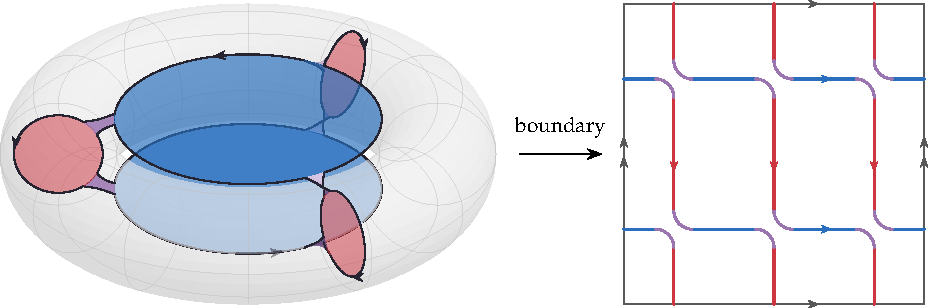
\includegraphics[width=0.7\textwidth]{torus-boundary.pdf}
  \caption{The minimal genus Seifert surface of $T(2,3)$, regarded as the composite cobordism from $T(0,0)$ to $T(2,3)$.}
  \label{fig:torus-boundary}
\end{figure}

Since these squares commute up to isotopy rel boundary, functoriality of $\mathfrak{gl}_N$ homology \cite{ehrig2018functoriality} shows that their induced maps on $\mathfrak{gl}_N$ homology commute. We can then define the Khovanov--Rozansky $\mathfrak{gl}_N$ homology of $T(\infty,\infty)$ as the stable limit \[\KR_N(T(\infty,\infty)):=\mathrm{colim}_{n,m\to\infty}q^{(m+n-mn)(N-1)}\KR_N(T(n,m)).\]By Lemma~\ref{lem:stosic_stable_range}, $\Sigma_i(n,m)$ induces an isomorphism in cohomological degree $h>-\min(m,n)$. The system therefore stabilizes in each cohomological degree along every path tending to $(\infty,\infty)$. Its colimit agrees with $\mathrm{colim}_{n\to\infty}\KR_N(T(n,\infty))$ along the cobordism maps defined by finite approximation, which itself also stabilizes in every fixed cohomological degree as $n\to\infty$. These stabilization results justify the limits of Poincar\'e series appearing in Appendix~\ref{app:Hilbert series}.

\section{Khovanov homology of \texorpdfstring{$T(n,n-1)$}{T(n,n-1)} and \texorpdfstring{$T(n,n)$}{T(n,n)}}\label{sec:unstable}
We now prove Theorem~\ref{thm:finite torus links and lasagna}.

\subsection{Khovanov homology of \texorpdfstring{$T(n,n-1)$}{T(n,n-1)}}\label{sbsec:T_n_n-1}
The key result that we use is the following.
\begin{lem}[{\cite{gorsky2023evaluations}}]\label{lem:GW_exact_tri}
For $n\ge2$, there are exact triangles
\begin{equation}\label{eq:GW_exact_tri_1}
\begin{tikzcd}[column sep=-5pt]
t^{2n-2}q^{6n-8}\Kh(T(n-2,n-2);\QQ)^{S_{n-2}}\ar[rr]&&\Kh(T(n,n);\QQ)^{S_n}\ar[ld]\\
&q^{n-1}\Kh(T(n,n-1);\QQ)\ar[lu,"\text{\emph{[1]}}"]&
\end{tikzcd}
\end{equation}
and
\begin{equation}\label{eq:GW_exact_tri_2}
\begin{tikzcd}[column sep=-5pt]
\Kh(T(n,n);\QQ)^{S_n}\ar[rr]&&t^{2n-2}q^{6n-4}\Kh(T(n-2,n-2);\QQ)^{S_{n-2}}\ar[ld,"\text{\emph{[1]}}"]\\
&q^{1-n}\Kh(T(n,n+1);\QQ)\ar[lu].&
\end{tikzcd}
\end{equation}
The horizontal maps in the triangles are each given by a dotted annulus that creates/annihilates two parallel strands, post-composed with symmetrization.
\end{lem}

By our grading convention, the Khovanov homology $\Kh(L)$ \cite{khovanov2000categorification} and the Khovanov--Rozansky $\mathfrak{gl}_2$ homology $\KR_2$ \cite{khovanov2008matrix} (called $\mathfrak{sl}_2$ homology there) over $\QQ$ are functorially related by $\Kh^{h,q}(L;\QQ)\cong(\KR_2^{-h,q}(L;\QQ))^*$. Lemma~\ref{lem:GW_exact_tri} follows from the $(\pm1)$-framed unknot case of \cite[Theorem~1.6.4]{ren2026khovanov}, which is in turn a consequence of \cite[Theorem~5.1 and Corollary~6.4]{gorsky2023evaluations} (and \cite[Proposition~1.4.3]{ren2026khovanov}).

Consequently, in terms of the Poincar\'e polynomials in the notation of Theorem~\ref{thm:finite torus links and lasagna}, we have bounds
\begin{equation}\label{eq:GW_inequalities}
I_n\le q^{n-1}A_n+t^{2n-2}q^{6n-8}I_{n-2},\ \ A_{n+1}\le q^{n-1}I_{n}+t^{2n-1}q^{7n-5}I_{n-2},
\end{equation}
where the inequalities are interpreted coefficientwise. If all these inequalities achieve equality, eliminating $I$ gives
$$A_n=q^{2n-4}A_{n-1}+t^{2n-4}q^{6n-12}A_{n-2}+t^{2n-3}q^{8n-16}A_{n-3},$$ as predicted by Theorem~\ref{thm:finite torus links and lasagna}(1).

By \cite[Theorem~4.7]{gorsky2013stable} and our resolution of \cite[Conjecture~4.9]{gorsky2013stable} in Appendix~\ref{app:Hilbert series}, with the correction noted there, one may check that the predicted sequence $A_n$, after appropriate renormalization, has coefficientwise limit equal to the Poincar\'e series of $\KR_2(T(\infty,\infty))$ described in \eqref{eqn:GOR fermionic series}. By the argument in Section~\ref{sec:stable torus homology}, the actual sequence $A_n$ leads to exactly the same coefficientwise limit. One may check that the initial values of $A_n$ agree with those in Theorem~\ref{thm:finite torus links and lasagna}. Hence, if any of the families of inequalities in \eqref{eq:GW_inequalities} were strict, one sees inductively that $A_n$ remains strictly smaller than predicted in some fixed nonnegative $t$-degree for all sufficiently large $n$, contradicting \eqref{eqn:GOR fermionic series} in the limit $n\to\infty$. This shows that both exact triangles \eqref{eq:GW_exact_tri_1} and \eqref{eq:GW_exact_tri_2} split, both inequalities in \eqref{eq:GW_inequalities} are equalities, and Theorem~\ref{thm:finite torus links and lasagna}(1) holds true.

\subsection{Symmetrized Khovanov homology of \texorpdfstring{$T(n,n)$}{T(n,n)}}
We have shown that \eqref{eq:GW_inequalities} achieves equalities. After checking Theorem~\ref{thm:finite torus links and lasagna}(2) for $n=0,1$ directly, the general case follows by using the first equality in \eqref{eq:GW_inequalities}.

\subsection{Khovanov homology of \texorpdfstring{$T(n,n)$}{T(n,n)}}
For any framed knot $K$, the rational Khovanov homology of its $n$-cables for various $n$ as an $S_n$-representation is determined by the symmetric-invariant part of these homology groups. This was implicit in the argument of \cite[Section~4.3]{ren2024lee}, and made more explicit in \cite[Proposition~1.4.3]{ren2026khovanov}; see also \cite[Theorem~1.1]{ritter2025computing}. On the level of Poincar\'e polynomials, this directly gives Theorem~\ref{thm:finite torus links and lasagna}(3).

\subsection{Khovanov skein lasagna module of \texorpdfstring{$\overline{\CP^2}$}{-CP2}}
By Manolescu--Neithalath's $2$-handlebody formula \cite[Theorem~1.1]{manolescu2022skein}, as recalled in \cite[Equations~(15) and~(28)]{ren2024khovanov}, the skein lasagna module of $\overline{\CP^2}$ in class $\epsilon=0,1$ is a colimit over cables of the $(-1)$-framed unknot along symmetrized dotted annulus creation maps. After mirroring and reorienting the cables, this is expressed in terms of $\Kh(T(2r+\epsilon,2r+\epsilon);\QQ)^{S_{2r+\epsilon}}$ and the horizontal maps in \eqref{eq:GW_exact_tri_1}, with the appropriate grading shifts. These maps are injective by Section~\ref{sbsec:T_n_n-1}, and their successive cokernels are shifted copies of $\Kh(T(n,n-1);\QQ)$. The colimit therefore retains every stage and adds precisely these cokernels. Summing their Poincar\'e polynomials, together with the initial empty-link or unknot term, gives \eqref{eqn:intro lasagna zero} and \eqref{eqn:intro lasagna one}. The formula for an arbitrary class follows from the change-of-orientation shift in \cite[Equation~(16)]{ren2024khovanov}, proving Theorem~\ref{thm:finite torus links and lasagna}(4).

\appendix

\section{Hilbert series}\label{app:Hilbert series}

In this Appendix, we compute the Poincar\'e series of $\KR_N(T(n,\infty))$ and $\KR_N(T(\infty,\infty))$ in Theorem~\ref{thm:stable Hilbert series}. The key ingredient is the splitting of the long exact sequence for $H_*(\cak_{r,l})$ into short exact sequences. It would be interesting to see if these series have arithmetic meanings; see, e.g., \cite{habiro2004cyclotomic,nahm2007conformal,zagier2007dilogarithm,zagier2010quantum}.

\subsection{\texorpdfstring{The Poincar\'e series of $T(n,\infty)$}{The Poincaré series of T(n,infinity)}}We compute the Poincar\'e series of the $\gl_N$ homology of $T(n,\infty)$. We keep the grading convention $(a,b,h)$ used in \eqref{eqn:link gradings} and denote the Poincar\'e series of $H_*(K_n)$ by
\[f_{n,N}(s,v,z)=\sum_{a,b,h\ge0}\dimm_{\QQ}H_h(K_n)_{a,b}s^av^bz^h,\]where we define $f_{0,N}=1$. Denote \[(A;v)_m=\prod_{i=0}^{m-1}(1-Av^i)\]with the understanding that $(A;v)_m=1$ when $m\le 0$. The polynomial ring $R_n$ has Poincar\'e series $(s;v)_n^{-1}$. Since $R_n$ is Noetherian and $K_n$ is finite free over $R_n$, each $H_h(K_n)$ is a finitely generated bigraded $R_n$-module. Its minimal bigraded free resolution is finite and has nonnegative shifts, so its Poincar\'e series is a finite alternating sum of terms $s^av^b/(s;v)_n$ with $a,b\ge0$. Multiplying $f_{n,N}$ by $(s;v)_n$ therefore gives a polynomial in $s,v,z$ with integer coefficients. We define \[g_{n,N}(s,v,z)=(s;v)_nf_{n,N}(s,v,z)\in\Z[s,v,z].\]%


\begin{thm}\label{thm:finite Hilbert series}The series $g_{n,N}$ is given by
\begin{equation}\label{eqn:finite Hilbert formula}
\begin{aligned}
g_{n,N}(s,v,z)&=\sum_{\substack{i\ge0,\ 0\le j\le N\\(N+1)i+j\le n}}(-1)^is^{Ni}v^{(2N+1)\binom{i}{2}+(N+j)i}(s;v)_i(-zs^N;v)_{Ni}\delta_j(sv^i,v,z)\\
&\ \cdot(-zs^{N+1}v^{(N+1)i+j};v)_{n-(N+1)i-j}\begin{bmatrix}n-Ni-j\\i\end{bmatrix}_v.
\end{aligned}
\end{equation}
Consequently, the Poincar\'e series of $\KR_N(T(n,\infty))$ is given by
\[
p_{n,N}(t,q)=f_{n,N}(q^2,t^{-2}q^2,t^{-1})=\frac{g_{n,N}(q^2,t^{-2}q^2,t^{-1})}{\prod_{i=0}^{n-1}(1-t^{-2i}q^{2i+2})}.
\]Here we define
\[\begin{bmatrix}A\\B\end{bmatrix}_v=\frac{(v;v)_A}{(v;v)_B(v;v)_{A-B}}\ (0\le B\le A),\]
and set it equal to zero otherwise, and let
\[
\delta_0(s,v,z)=1,\delta_1(s,v,z)=-s^N(1+zs),\delta_j(s,v,z)=-(1-s)s^Nv^{j-1}(-zs^N;v)_{j-1}\ (2\le j\le N).
\]

\end{thm}

To compute $f_{n,N}$ or $g_{n,N}$, we relate them with the Poincar\'e series of the homology of the auxiliary complexes $H_*(\cak_{r,l})$. Recall that there is a weight grading on $\cak_{r,l}$ defined in \eqref{eqn:weight grading}, and denote the Poincar\'e series of $H_*(\cak_{r,l})$ by
\[h_{r,l}(w,z)=\sum_{b,h\ge0}\dimm_{\QQ}H_h(\cak_{r,l})_bw^bz^h.\]For $0\le m\le r$, the generators $u_i$ and $\xi_i$ of $K_m$ have weights $r-i$ and $Nr-i$, respectively, under the isomorphism in Proposition~\ref{prop:Krl in terms of Km}. Hence $f_{m,N}$ is related to $h_{r,Nr-m}$ by
\begin{equation}\label{eqn:Hilbert reversal}
h_{r,Nr-m}(w,z)=\frac{\prod_{j=Nr+1}^{(N+1)r-m}(1+zw^j)}{\prod_{i=1}^{r-m}(1-w^i)}f_{m,N}(w^r,w^{-1},z).
\end{equation}We compute the Poincar\'e series using the following proposition.

\begin{prop}
For $r,l\ge1$ and $l<Nr$, the long exact sequence \eqref{eqn:long exact sequence in homology} breaks into short exact sequences
\[0\to H_h(\cak_{r-1,l})\langle l\rangle\xrightarrow{\delta}H_h(\cak_{r,l})\xrightarrow{J_*}H_h(\cak_{r,l-1})\to0,\]
where $\langle l\rangle$ denotes a weight shift by $l$. Thus
\begin{equation}\label{eqn:auxiliary Hilbert recurrence}
h_{r,l}(w,z)=h_{r,l-1}(w,z)+w^lh_{r-1,l}(w,z).
\end{equation}
\end{prop}

\begin{proof}
Theorem~\ref{thm:2 parameter Koszul generation} and \eqref{eqn:J preserves tail classes} imply that $J_*$ is surjective in every Koszul degree, so the long exact sequence \eqref{eqn:long exact sequence in homology} breaks into short exact sequences. Since $\pi$ removes the factor $\chi_l$ of weight $l$ and Koszul degree $1$, the connecting map $\delta$ has weight $l$ and Koszul degree zero, and \eqref{eqn:auxiliary Hilbert recurrence} follows.
\end{proof}

\begin{prop}The series $g_{n,N}(s,v,z)$  is determined by the following initial conditions and recurrence relations.
For $1\le n\le N+1$,
\begin{equation}\label{eqn:initial Hilbert numerators}
g_{n,N}(s,v,z)=\frac{1}{z}\left((1+z)\prod_{j=1}^{n-1}(1+zs^{N+1}v^j)-\prod_{i=0}^{n-1}(1+zs^Nv^i)\right).
\end{equation}
For $n\ge N$,
\begin{equation}\label{eqn:Hilbert numerator recurrence}
g_{n+1,N}(s,v,z)=(1+zs^{N+1}v^n)g_{n,N}(s,v,z) \ -(1-s)s^Nv^n(-zs^N;v)_Ng_{n-N,N}(sv,v,z).
\end{equation}
\end{prop}

\begin{proof}
The short exact sequences \[0\to Z_*(K_n)\to(K_n)_*\xrightarrow{d}B_{*-1}(K_n)\to0\]and\[0\to B_*(K_n)\to Z_*(K_n)\to H_*(K_n)\to0\]yield the following relations among their Poincar\'e series:
\[h_{K_n}=h_{Z_*(K_n)}+zh_{B_*(K_n)},\ f_{n,N}=h_{Z_*(K_n)}-h_{B_*(K_n)}.\]For $1\le n\le N+1$, Proposition~\ref{prop:cycles in short Koszul complexes} gives \[h_{Z_*(K_n)}=\frac{\prod_{j=1}^{n-1}(1+zs^{N+1}v^j)}{(s;v)_n},\ h_{K_n}=\frac{\prod_{i=0}^{n-1}(1+zs^Nv^i)}{(s;v)_n}.\]Hence, $zf_{n,N}=(1+z)h_{Z_*(K_n)}-h_{K_n}$, which proves \eqref{eqn:initial Hilbert numerators}.

Let $P(s,v,z)$ be the difference between the left and right sides of \eqref{eqn:Hilbert numerator recurrence}. This is a polynomial, and plugging \eqref{eqn:Hilbert reversal} into \eqref{eqn:auxiliary Hilbert recurrence} at $l=Nr-n$ gives $P(w^r,w^{-1},z)=0$ for every $r\ge n+1$. For $r>\deg_vP$, distinct monomials $s^av^b$ in $P$ give distinct powers $w^{ra-b}$, so their coefficients in $\QQ[z]$ must all vanish. Hence $P=0$, which proves the recursive relation.
\end{proof}

We can further solve the recurrence relation \eqref{eqn:Hilbert numerator recurrence}.

\begin{proof}[Proof of Theorem~\ref{thm:finite Hilbert series}]
For fixed $v$ and $z$, we define generating series
\[\ell(X;s)=\sum_{n\ge0}\frac{g_{n,N}(s,v,z)}{(-zs^{N+1};v)_n}X^n,\ \beta(X;s)=\sum_{j=0}^N\frac{\delta_j(s,v,z)}{(-zs^{N+1};v)_j}X^j.\]
The initial conditions \eqref{eqn:initial Hilbert numerators} and recurrence \eqref{eqn:Hilbert numerator recurrence} give
\[\ell(X;s)=\frac{\beta(X;s)}{1-X}-\frac{(1-s)s^Nv^NX^{N+1}(-zs^N;v)_N}{(1-X)(-zs^{N+1};v)_{N+1}}\ell(vX;sv).\]
Iterating this gives
\begin{equation}\label{eqn:iterated length series}
\ell(X;s)=\sum_{i\ge0}\frac{(-1)^iX^{(N+1)i}s^{Ni}v^{(2N+1)\binom{i}{2}+Ni}(s;v)_i(-zs^N;v)_{Ni}}{(X;v)_{i+1}(-zs^{N+1};v)_{(N+1)i}}\beta(v^iX;sv^i).
\end{equation}
Now \eqref{eqn:finite Hilbert formula} follows from comparing the coefficients of $X^n$ in \eqref{eqn:iterated length series}. The assertion about the Poincar\'e series of $\KR_N(T(n,\infty))$ follows from \eqref{eqn:link gradings}, which translates the gradings.
\end{proof}

\subsection{\texorpdfstring{The Poincar\'e series of $T(\infty,\infty)$}{The Poincaré series of T(infinity,infinity)}}

We now compute the Poincar\'e series of the $\gl_N$ homology of $T(\infty,\infty)$ by taking the limit of the finite-strand formula and rewriting it as a sum with nonnegative coefficients. Set
\[f_{\infty,N}(s,v,z)=\lim_{n\to\infty}f_{n,N}(s,v,z),\]
and write $(A;v)_\infty=\prod_{i\ge0}(1-Av^i)$. Taking the limit in Theorem~\ref{thm:finite Hilbert series} using
\[\lim_{n\to\infty}\begin{bmatrix}n-Ni-j\\i\end{bmatrix}_v=\frac1{(v;v)_i}\]
gives
\begin{equation}\label{eqn:strand bosonic formula}
\begin{aligned}
f_{\infty,N}(s,v,z)&=\frac1{(s;v)_\infty}\sum_{i\ge0}\sum_{j=0}^N\frac{(-1)^is^{Ni}v^{(2N+1)\binom{i}{2}+(N+j)i}(s;v)_i(-zs^N;v)_{Ni}}{(v;v)_i}\\
&\ \cdot\delta_j(sv^i,v,z)(-zs^{N+1}v^{(N+1)i+j};v)_\infty.
\end{aligned}
\end{equation}

The expression \eqref{eqn:strand bosonic formula} already gives a closed formula for the Poincar\'e series of $\KR_N(T(\infty,\infty))$. Following \cite[Section 4.2]{gorsky2013stable}, we can rewrite it as a ``Fermionic'' sum with nonnegative coefficients.

To expand the infinite products in \eqref{eqn:strand bosonic formula}, we use the binomial identity
\[\frac{(-AX;v)_\infty}{(X;v)_\infty}=\sum_{\ell\ge0}\frac{(-A;v)_\ell}{(v;v)_\ell}X^\ell.\]With $A=zs^Nv^{Ni+j}$ and $X=sv^i$, this gives
\begin{equation}\label{eqn:binomial expansion}
\frac{(-zs^{N+1}v^{(N+1)i+j};v)_\infty}{(sv^i;v)_\infty}=\sum_{\ell\ge0}\frac{(-zs^Nv^{Ni+j};v)_\ell}{(v;v)_\ell}s^\ell v^{i\ell}.
\end{equation}
The finite product on the right depends on $s$ and $z$ only through $zs^N$. We therefore set $y=zs^N$ to obtain an expansion in $s$ with $y$ fixed, and define $c_{N,k}(y,v)$ by
\begin{equation}\label{eqn:charge series}
f_{\infty,N}(s,v,ys^{-N})=\sum_{k\ge0}s^kc_{N,k}(y,v).
\end{equation}
Here $k=a-Nh\ge 0$ since the generators $u_i$ and $[\mu_j]$ have $(a,h)$ bigradings $(1,0)$ and $(N+1,1)$ respectively. Taking coefficients in \eqref{eqn:strand bosonic formula} using \eqref{eqn:binomial expansion}, we obtain the following finite alternating sum:
\begin{equation}\label{eqn:alternating charge formula}
\begin{aligned}
c_{N,k}(y,v)&=\sum_{Nj+\ell=k}\frac{(-1)^jv^{jk+\binom{j}{2}}(-y;v)_k}{(v;v)_j(v;v)_\ell}\\
&\ -y\sum_{Nj+\ell=k-1}\frac{(-1)^jv^{j(k+N)+\binom{j+1}{2}}(-y;v)_{Nj}(-yv^{Nj+1};v)_\ell}{(v;v)_j(v;v)_\ell}\\
&\ -\sum_{Nj+\ell=k-N}\frac{(-1)^jv^{jk+\binom{j+1}{2}}(-y;v)_{Nj}(-yv^{Nj+1};v)_\ell}{(v;v)_j(v;v)_\ell}\\
&\ -\sum_{\substack{Nj+\ell=k-N\\2\le i\le N}}\frac{(-1)^jv^{j(k+i)+\binom{j}{2}+\ell+i-1}(-y;v)_{Nj+\ell+i-1}}{(v;v)_j(v;v)_\ell}.
\end{aligned}
\end{equation}
All sums are over nonnegative $j,\ell$. For $0\le k<N-1$, the only terms that contribute are those with $j=0$ in the first two sums, so
\[c_{N,k}(y,v)=\frac{(-yv;v)_k}{(v;v)_k},\ 0\le k<N-1.\]

We rewrite \eqref{eqn:alternating charge formula} as a sum with nonnegative coefficients.

\begin{thm}\label{thm:fermionic formula}
For $0\le k<N-1$, $c_{N,k}(y,v)=(-yv;v)_k/(v;v)_k$. For $1\le i\le N$, define
\[\gamma_{N,i,k}(v)=\sum_{\substack{n_1\ge\dots\ge n_N=0\\\sum_{j=1}^{N-1}n_j=k}}\frac{v^{\sum_{j=1}^{N-1}n_j(n_j-1)+\sum_{j=i}^{N-1}n_j}}{\prod_{j=1}^{N-1}(v;v)_{n_j-n_{j+1}}}.\]
Then we have
\begin{equation}\label{eqn:fermionic formula}
c_{N,k}(y,v)=(-y;v)_{k-N+1}\gamma_{N,N,k}(v)+y\sum_{i=1}^{N-1}v^{k-i}(-y;v)_{k-i}\gamma_{N,i,k}(v)
\end{equation}for $k\ge N-1$.
In particular, $c_{N,k}$ has nonnegative integer coefficients in $y$ and $v$. Consequently, the Poincar\'e series $p_{\infty,N}(t,q)$ of the normalized unreduced $\gl_N$ homology of $T(\infty,\infty)$ is given by
\[p_{\infty,N}(t,q)=\sum_{k\ge0}q^{2k}c_{N,k}(t^{-1}q^{2N},t^{-2}q^2).\]
\end{thm}

\begin{proof}
For $N=1$, the formula follows from $H_*(K_n)=\QQ$ and the empty-sum and empty-product conventions in the definition of $\gamma_{1,1,k}$. In the remainder of the proof, assume $N\ge2$.

We first write the sums $\gamma_{N,i,k}$ as alternating sums. For $1\le i\le N$, let
\[\gamma_{N,i}(s,v)=\sum_{k\ge0}s^k\gamma_{N,i,k}(v),\ \gamma_{N,0}=0.\]
Let $\mathcal P_{N,i;k}$ be the set of partitions $\lambda=(\lambda_1\ge\dots\ge\lambda_k\ge0)$ with at most $i-1$ zero parts and $\lambda_j-\lambda_{j+N-1}\ge2$ for $1\le j\le k-N+1$. By \cite[Equation~(2)]{fortin2004generating}, we have
\[\gamma_{N,i}(s,v)=\sum_{k\ge0}\left(\sum_{\lambda\in\mathcal P_{N,i;k}}v^{\lambda_1+\dots+\lambda_k}\right)s^k.\]
Here $\gamma_{N,i}(s,v)=F_{N,i}(s/v;v)$ in the notation of \cite{fortin2004generating}. A partition counted in $\gamma_{N,i}-\gamma_{N,i-1}$ has exactly $i-1$ zero parts. The map
\[(\lambda_1,\dots,\lambda_k)\mapsto(\lambda_1-1,\dots,\lambda_{k-i+1}-1)\]
removes these zeros and subtracts one from each remaining part. The image has at most $N-i$ zero parts, since the original partition has at most $N-1$ parts equal to zero or one. This bijection gives
\begin{equation}\label{eqn:Gordon recurrence}
\gamma_{N,i}(s,v)-\gamma_{N,i-1}(s,v)=s^{i-1}\gamma_{N,N-i+1}(sv,v),\ \gamma_{N,i}(0,v)=1\ (1\le i\le N).
\end{equation}

The recurrence \eqref{eqn:Gordon recurrence} and initial values determine the series uniquely by inducting on the $s$-degree simultaneously for all $i$. The solution is
\begin{equation}\label{eqn:Gordon single sum}
\gamma_{N,i}(s,v)=\sum_{j\ge0}\frac{(-1)^js^{Nj}v^{(2N+1)\binom{j}{2}+Nj}}{(v;v)_j(sv^j;v)_\infty}\left(v^{(1-i)j}-s^iv^{(i+1)j}\right)\ (0\le i\le N).\end{equation}Indeed, the right-hand side vanishes for $i=0$ and has value $1$ at $s=0$ for $i\ge1$. Subtracting the expressions for $i$ and $i-1$ gives two sums, with factors $1-v^j$ and $1-sv^j$, respectively. Cancelling these factors against the denominators and reindexing the first sum by $j\mapsto j+1$ gives $s^{i-1}$ times the expression for $\gamma_{N,N-i+1}(sv,v)$, as required by \eqref{eqn:Gordon recurrence}.

Taking the coefficient of $s^k$ in \eqref{eqn:Gordon single sum} gives
\begin{equation}\label{eqn:Gordon fixed charge}
\gamma_{N,i,k}(v)=\sum_{j=0}^{\lfloor k/N\rfloor}\frac{(-1)^jv^{jk+\binom{j+1}{2}}}{(v;v)_j(v;v)_{k-Nj}}\bigl(v^{-ij}-(v^{k-Nj-i+1};v)_i\bigr).
\end{equation}
The product in the second term vanishes when $k-Nj<i$.

For $k\ge N-1$, write
\[S_k(w)=\sum_{\ell=0}^{N-2}(-yv^{k+1-N};v)_\ell w^{\ell-N}.\]
Insert \eqref{eqn:Gordon fixed charge} into the right-hand side of \eqref{eqn:fermionic formula}. Subtracting \eqref{eqn:alternating charge formula} then gives
\[\begin{aligned}
&\frac{(-y;v)_{k-N+1}\gamma_{N,N,k}+y\sum_{i=1}^{N-1}v^{k-i}(-y;v)_{k-i}\gamma_{N,i,k}-c_{N,k}}{(-y;v)_{k-N+1}}\\
&\ =\sum_{j=1}^{\lfloor k/N\rfloor}\frac{(-1)^jv^{jk+\binom{j+1}{2}}S_k(v^j)}{(v;v)_{j-1}(v;v)_{k-Nj}}+\sum_{j=0}^{\lfloor k/N\rfloor-1}\frac{(-1)^jv^{(j+1)k+\binom{j+2}{2}}S_k(v^{j+1})}{(v;v)_j(v;v)_{k-N(j+1)}}=0
\end{aligned}\]by replacing $j$ with $j+1$ in the second sum. This proves \eqref{eqn:fermionic formula}.

The inclusions $K_n\to K_{n+1}$ preserve the differential and the three gradings $(a,b,h)$. The chain groups of weight $b$ are unchanged once $n>b$, so the coefficientwise limit $f_{\infty,N}$ exists and is the trigraded Poincar\'e series of $\mathrm{colim}_{n\to\infty}H_*(K_n)$. By the stabilization in each cohomological degree proved in Section~\ref{sec:stable torus homology},
\[p_{\infty,N}(t,q)=\lim_{n\to\infty}p_{n,N}(t,q).\]By Theorem~\ref{thm:finite Hilbert series} and \eqref{eqn:charge series}, we have
\[p_{\infty,N}(t,q)=f_{\infty,N}(q^2,t^{-2}q^2,t^{-1})=\sum_{k\ge0}q^{2k}c_{N,k}(t^{-1}q^{2N},t^{-2}q^2).\qedhere\]
\end{proof}

For $N=2$, we have
\begin{equation}\label{eqn:GOR fermionic series}
f_{\infty,2}(s,v,ys^{-2})=\sum_{i\ge0}\frac{s^iv^{i(i-1)}(-yv;v)_i}{(v;v)_i}\left(1+ys^2v^{4i+2}\right),
\end{equation}
which confirms  \cite[Conjecture~4.9]{gorsky2013stable} with the following understanding. Their Fermionic sum $A(a,q,t)$ is our $\sum_{k\ge0}q^{2k}c_{2,k}(a^2t,t^2q^2)$, and the Bosonic sum $B(a,q,t)$ is our $f_{\infty,2}(q^2,t^2q^2,a^2tq^{-4})$ after omitting the middle summand at $p=0$ in their expression. After this, both series begin with
\[1+q^2+q^4t^2+a^2q^4t^3+q^6t^4+a^2q^6t^5+O(q^8).\]

\bibliographystyle{amsra}
\bibliography{ref}

\end{document}
